\begin{tcolorbox}[colback=red!5!white,colframe=red!75!black,title=Important note]
    In this lab, an incompatibility meant that instead
    of using the base GPG program, the alternative \textbf{GnuPG1} was used.
    Therefore, commands use the phrase "gpg1" instead of "gpg".
\end{tcolorbox}

This lab expanded on the concepts of asymmetric encryption through the use of\newline
GPG/GnuPG (GNU Privacy Guard) to produce, sign and verify public and private keys.\\

\section{Creating test users}\label{sec:testUsers}
For this lab, two test users were created and used to execute the necessary commands.

\subsection{Elevating the terminal}\label{subsec:sudo}
To add users to the system, administrative privileges are required.
To gain the necessary privileges, the command "sudo -s" or "sudo bash" can be entered
(both commands are functionally identical) which will change the terminal to be at root level.

\begin{figure}[H]
    \centering
    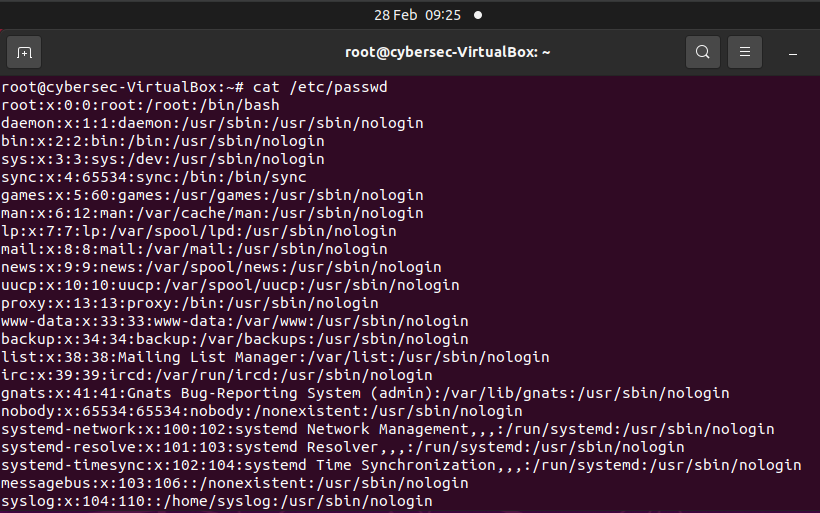
\includegraphics[width=.9\linewidth]{lab2/1}
    \caption{Elevating the terminal.}
    \label{fig:sudo}
\end{figure}

\subsection{Creating Bob and Alice}\label{subsec:createUsers}
With the elevated privileges gained from being a superuser, it is now possible to add users to the system using
"adduser" followed by the given username.
A password for the user will then be necessary, followed by optional information such as phone
numbers, which are left blank for this lab.

\begin{figure}[H]
    \centering
    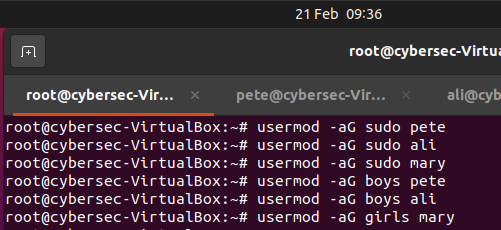
\includegraphics[width=.49\linewidth]{lab2/2}
    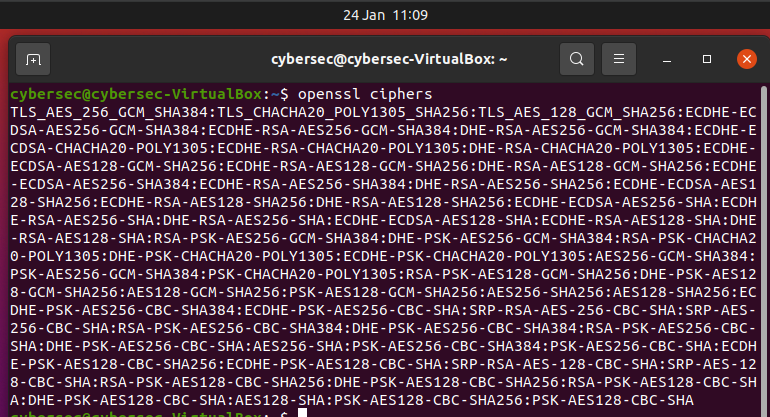
\includegraphics[width=.49\linewidth]{lab2/3}
    \caption{Creating users 'bob' and 'alice'.}
    \label{fig:createBob}
\end{figure}

%\begin{figure}[H]
%    \centering
%    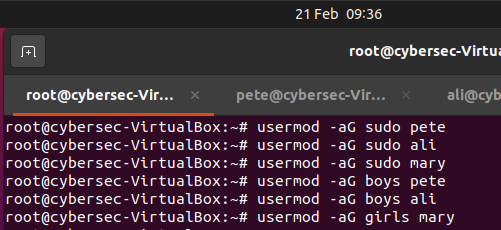
\includegraphics[width=.6\linewidth]{lab2/2}
%    \caption{Creating user 'alice'.}
%    \label{fig:createAlice}
%\end{figure}

For ease of access, multiple terminal tabs can be open at a time, so I elected to use one for the superuser root,
and one each for Bob and Alice.

\begin{figure}[H]
    \centering
    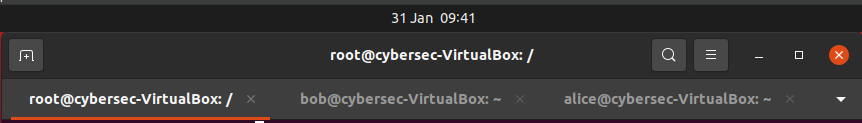
\includegraphics[width=.9\linewidth]{lab2/4}
    \caption{Multiple terminal tabs.}
    \label{fig:terminalTabs}
\end{figure}

I also added these new users to the "sudo" group, allowing them to also use the sudo command to execute commands
with elevated permissions.

\begin{figure}[H]
    \centering
    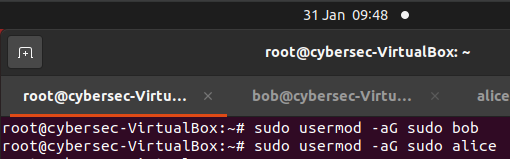
\includegraphics[width=.8\linewidth]{lab2/5b}
    \caption{Adding bob and alice to sudo.}
    \label{fig:sudoAdd1}
\end{figure}

%\begin{figure}[H]
%    \centering
%    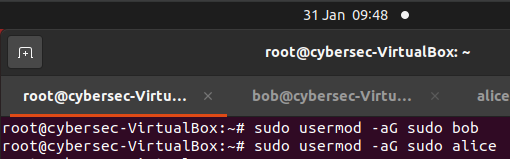
\includegraphics[width=.8\linewidth]{lab2/5b}
%    \caption{Adding bob and alice to sudo.}
%    \label{fig:sudoAdd2}
%\end{figure}

% ^ Unnecessary because this can be one figure.

It is possible to switch the active terminal user using the command "su" followed by the account to switch to,
and then the password of the given account.

\begin{figure}[H]
    \centering
    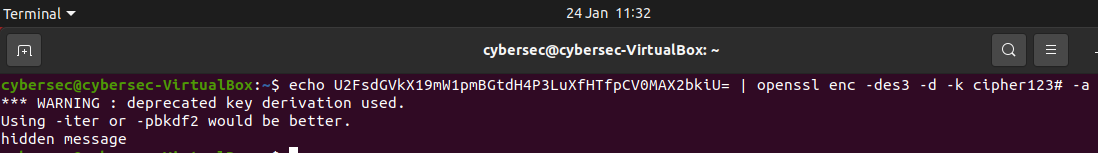
\includegraphics[width=.9\linewidth]{lab2/5c}
    \caption{Switching the active terminal user.}
    \label{fig:suBobAlice}
\end{figure}

Note the prompt about running commands as an administrator,
which signifies that they were successfully added to the sudo group.


\pagebreak

\section{Exchanging encrypted files over an insecure channel}\label{sec:tmpExchange}
\begin{tcolorbox}[colback=orange!5!white,colframe=orange!75!black]
    For this section, assume that all commands have been executed on \textbf{both} the Bob and Alice
    user accounts unless stated otherwise.
\end{tcolorbox}
On standard Linux distributions, the /tmp directory is a public directory accessible to all users.
For this reason, it is therefore insecure, as every user on the system can read the files placed there.\footnote{However, they cannot update/change them without sudo permissions.}
To transfer files across insecure channels such as /tmp/, they should first be encrypted so that
they can only be read and/or used by their intended recipient.
Therefore, GNU Privacy Guard (GPG hereafter) can be used to generate and store public
and private asymmetric keys.

\subsection{Generating public/private key-pairs}\label{subsec:generating-private-keys}

To generate a private key, the command "gpg1 --gen-key" can be used.

\begin{figure}[H]
    \centering
    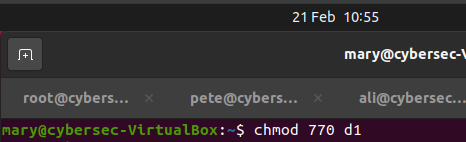
\includegraphics[width=.5\linewidth]{lab2/9}
    \caption{Generating a private key.}
    \label{fig:GPGgen}
\end{figure}

This will open a submenu where the user can select the kind of key they wish to generate,
as well as the size and expiry date of the key.
Once this is established, they must create a user ID if they didn't already have one,
consisting of their full name, email address and an optional comment.
While the key generates, the user is prompted to perform random inputs such as moving the mouse
and typing on the keyboard to enhance the randomness of the generated key.
A key was also generated for Alice.

\pagebreak

\subsection{Exporting public keys}\label{subsec:exporting-public-keys}
It is possible to export the public keys from the generated key-pairs using GPG's export command.

\begin{figure}[H]
    \centering
    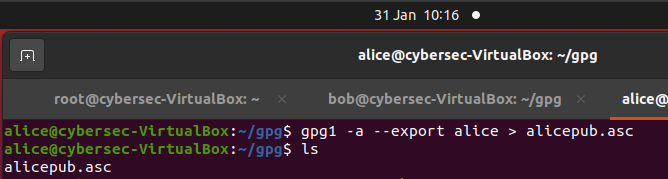
\includegraphics[width=.9\linewidth]{lab2/11b}
    \caption{Exporting Alice's public key.}
    \label{fig:GPGexport}
\end{figure}

\noindent This exports the public key in ASCII format (due to the use of the -a flag) to the file "alicepub.asc".
This can be seen by using "ls" to show the files in the directory.\footnote{The file can be read using "cat alicepub.asc", but it is a 2048-bit key, so it would completely fill the terminal window.}
Because this is Alice's \textbf{public} key, we are comfortable sharing this to the public /tmp/ directory where all
users can see it.

\begin{figure}[H]
    \centering
    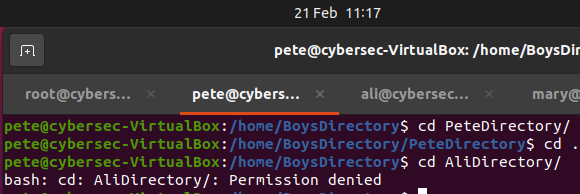
\includegraphics[width=.9\linewidth]{lab2/13}
    \caption{Copying Alice's public key to /tmp.}
    \label{fig:alicePubTmp}
\end{figure}


\subsection{Importing and signing public keys}\label{subsec:importing-public-keys}
Now that Alice's public key is in /tmp, Bob can copy this to his own directory and import it using GPG\@.

\begin{figure}[H]
    \centering
    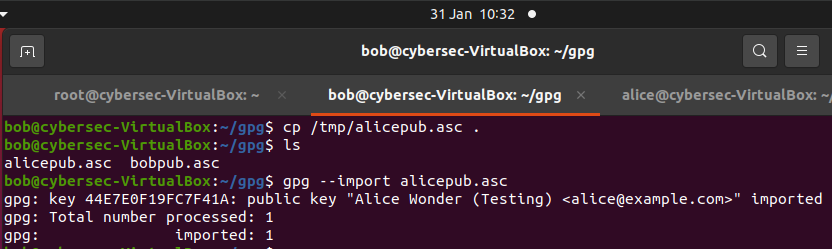
\includegraphics[width=.9\linewidth]{lab2/14}
    \caption{Importing Alice's public key as Bob.}
    \label{fig:importAlice}
\end{figure}

\pagebreak

\noindent Bob can then \textbf{sign} this key, verifying that he trusts that this key does belong to Alice.
This is done by editing Alice's key as Bob, signing it, and then saving this.

\begin{figure}[H]
    \centering
    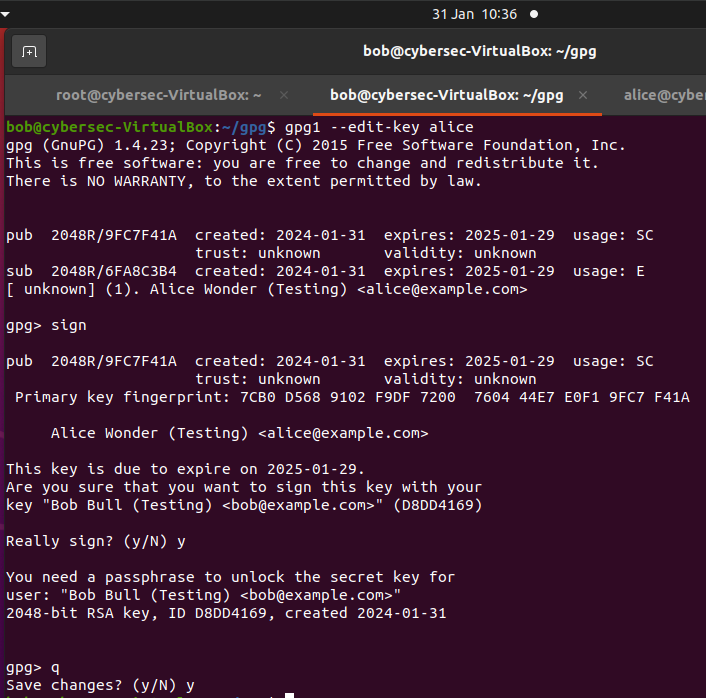
\includegraphics[width=.7\linewidth]{lab2/15}
    \caption{Bob signing Alice's public key.}
    \label{fig:signAliceKey}
\end{figure}

\pagebreak

\subsection{Encrypting and decrypting data}\label{subsec:encrDecr}
Now that Alice and Bob have their key-pairs generated, they can transfer asymmetrically encrypted data to each other.
This was tested by making a file, encrypting it using Alice's public key, and copying it to the /tmp directory.

\begin{figure}[H]
    \centering
    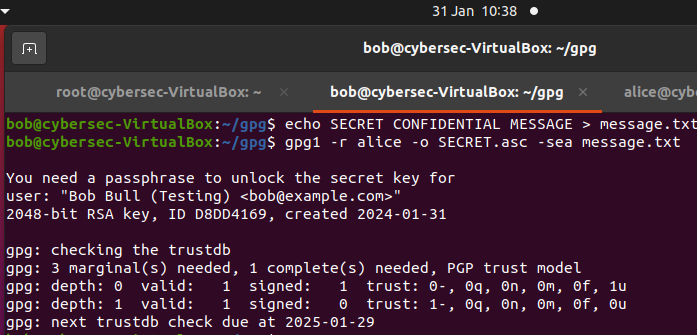
\includegraphics[width=.9\linewidth]{lab2/16}
    \caption{Making a file and encrypting it using Alice's public key.}
    \label{fig:encLab2Msg}
\end{figure}

This command can be broken down to its components:
\begin{itemize}
    \item -r alice - Sets Alice as the recipient of the file by using her public key.
    \item -o SECRET.asc - Outputs the encrypted data to SECRET.asc.
    \item -sea message.txt - Sign and encrypt the contents of message.txt in ASCII format.
\end{itemize}

\begin{figure}[H]
    \centering
    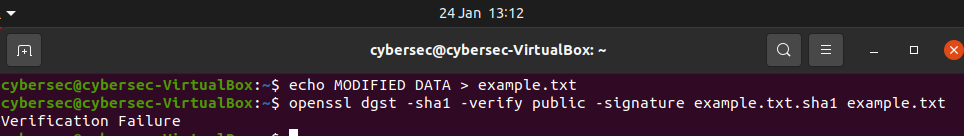
\includegraphics[width=.9\linewidth]{lab2/17}
    \caption{Copying the encrypted file to /tmp with the name "secret\_to\_alice.asc".}
    \label{fig:copyLab2Msg}
\end{figure}

Alice can then decrypt "secret\_to\_alice.asc" and output the results to "message.txt", where they can then
be read in human-legible form.

\begin{figure}[H]
    \centering
    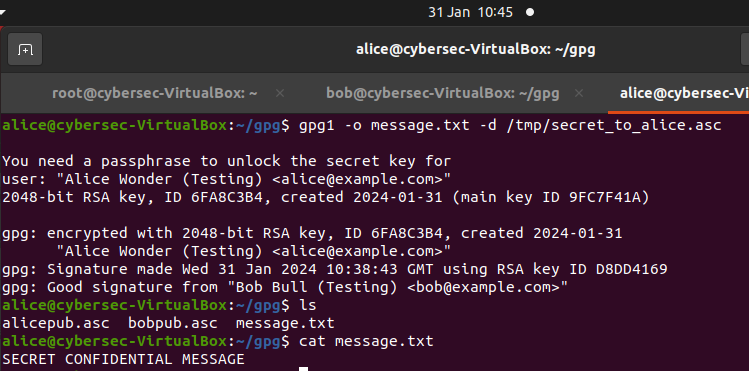
\includegraphics[width=.9\linewidth]{lab2/18}
    \caption{Decrypting the encrypted message and reading it.}
    \label{fig:decryptLab2Msg}
\end{figure}
